%=================================================================%
%
% Author:  Aaron S. Tamashiro        
%          Graduate Research Assistant
%          Oregon State University
%          September, 2017
%
% LaTex Styling by Brenton Ching
%
% Description:
%          This is the thesis "root" file which
%          includes:
%             - preamble
%             - style packages
%             - "includes" of the files
% 
% Outline:

%
%=================================================================%

%==========%
% Preamble %
%==========%

\documentclass[12pt,letterpaper]{article}

\usepackage{standard-Tony} % Tony's standard.sty fixes the table of contents
%\usepackage{standard}         % Tells LaTeX to use "standard.sty"
			      % *** does NOT require modifications

\usepackage{personal}         % Tells LaTeX to use "personal.sty"
			      % *** user can modify this file
			      
%\usepackage{graphicx}	% Added by IMD

\usepackage{paralist}	% Added by IMD

% Added by JRH

% To use Tikz
\usepackage{tikz}
\usetikzlibrary{patterns}
\usetikzlibrary{shapes.misc}

% To use \FloatBarrier
\usepackage{placeins}

% To use subfigures
\usepackage{subcaption}
\usepackage{caption}

% To use longtables
\usepackage{longtable}
\usepackage{tabu}

% To use quotations \say
\usepackage{dirtytalk}

% for 'landscape' environment
\usepackage{pdflscape} 

% make the degree symbol with $^{\circ}$
\usepackage{gensymb}

% Dummy text
\usepackage{lipsum}


\begin{document} 

%=================================================================%

                     %==========================%
                     %    Build the document    %
                     %==========================%

\SetDoubleSpace        % Start double-spacing

%==========%
% Abstract %
%==========%

%=================%
% Section:        %
%    Abstract     %
%=================%

\begin{center} AN ABSTRACT OF THE THESIS OF  \end{center}

\thispagestyle{empty}

\belowSecSkip

\ResetSingleSpace

\noindent \underline{Aaron S. Tamashiro} for the degree of 
	  \underline{Master of Science} in
	  \underline{Nuclear Engineering} presented on 
	  \underline{\myDefenseDate}. \\
	  Title: \underline{Thesis Template} \\
      \hfill\underline{Use multiple lines if title doesn't fit in one}
	%\hfill\underline{Deterministic Phonon Transport Simulations}.

\vskip0.3in

\noindent Abstract approved: \hspace{0.25in} \hrulefill\




	  
\noindent \hspace{3.25in} Todd S. Palmer \hfill

\vskip0.25in


% Begin abstract text %

\ResetDoubleSpace

\noindent
	\indent \lipsum[2-4]
    \indent \lipsum[1]
    
% * <reynolaa@oregonstate.edu> 2018-12-05T02:49:14.097Z:
% 
% I'd structure this chronologically: what's been done, where improvement is needed, and how your work makes improvements. Without being an expert in this stuff, I edited this with what I'd do. Just spitballing.
% 
% ^.
    
\thispagestyle{empty}


%===========%
% Copyright %
%===========%

%================%
% Section:       %
%   Copyright    %
%================%

\thispagestyle{empty}

\belowSecSkip

\vspace*{2.5in}

\begin{center}
	\copyright Copyright by Aaron S. Tamashiro \\
	\myDefenseDate \\
	All Rights Reserved
\end{center}



%============%
% Title page %
%============%

\ResetSingleSpace      % ... back to single-spacing

%============%
% Title page %
%============%

\thispagestyle{empty}

% Set spacing for title line.
\setlength{\baselineskip}{21pt}

\begin{center}
{
   \myTitleName
\\ \vspace{0.25in}
   by
\\ \vspace{0.25in}
   Aaron S. Tamashiro
\\ \vspace{1.0in}
   A THESIS
\\ \vspace{0.25in}
   submitted to
\\ \vspace{0.25in}
   Oregon State University
\\ \vspace{1.0in}
   in partial fulfillment of
\\
   the requirements for the
\\
   degree of
\\ \vspace{0.25in}
   Master of Science
\\ \vspace{1.0in}
   Presented \myDefenseDate
\\ 
   Commencement \myCommenceDate
}
\end{center}

% Re-set spacing for rest of document.
\addtolength{\baselineskip}{-7pt}




%==========%
% Approval %
%==========%

%===============%
% Approval page %
%===============%

\thispagestyle{empty}

\noindent \underline{Master of Science} thesis of
	  \underline{Aaron S. Tamashiro} presented on
	  \underline{\myDefenseDate}.

\vspace{0.5in}

\noindent APPROVED:

\vspace{1.0in}

\noindent \hrulefill 

\noindent Major Professor, representing Nuclear Engineering

\vspace{1.0in}

\noindent \hrulefill

\noindent Head of the School of Nuclear Science and Engineering

\vspace{1.0in}

\noindent \hrulefill

\noindent Dean of the Graduate School

\vspace{1.0in}

\noindent I understand that my thesis will become part of the
	  permanent collection of Oregon State University
	  libraries.  My signature below authorizes release 
	  of my thesis to any reader upon request.

\vspace{0.9in}

\noindent \hrulefill 

\begin{center}
   Aaron S. Tamashiro, Author
\end{center}



%=================%
% Acknowledgement %
%=================%

\ResetDoubleSpace      % ... back to double-spacing

%=================%
% Acknowledgements %
%=================%

\begin{center}
\section*{\mdseries{ACKNOWLEDGEMENTS}}
\label{sec:ack}
\end{center}

\thispagestyle{empty}

\noindent
	\indent \lipsum[1-2]



\thispagestyle{empty}


%======================================================%
% Table of Contents / List of Figures / List of Tables %
%======================================================%

% This formats the pagestyle.

%\pagestyle{startlists}\clearpage 

% The toc, lof, and lot must be ordered so that the list
% which is only ONE page is first.
%\setlength{\topmargin}{-0.7in}
%\setlength{\textheight}{8.7in}
\tableofcontents\clearpage

\listoffigures\clearpage

\listoftables\clearpage

% This re-formats the pagestyle.

%\pagestyle{endlists}\clearpage 

% This re-re-formats the pagestyle.  Unfortunately, it
% also creates an empty (blank) page.

\thispagestyle{empty}
\section*{}
\clearpage

\pagestyle{myheadings}

%==============%
% Introduction %
%==============%

%=================%
% Section:        %
%    Introduction %
%=================%

\ResetSingleSpace

\begin{center}
{\textbf{
Thesis Template}}
\end{center}

\ResetDoubleSpace

\vskip0.25in

\begin{center}
\section{INTRODUCTION}
\label{sec:Intro}
\end{center}

\setcounter{page}{1}
\thispagestyle{empty}

\vskip-0.1in

%%%%%%%%%%%%%%%%%%%%%%%%%%%%%%%%%%%%%%%%%%%%%%%%%%
\noindent
    According to Tamashiro, my thesis must follow the guidelines set by the graduate school \cite{Tamashiro4}. I am showing you some reference examples \cite{Tamashiro1}. At the end of this template, you will see how my references are labeled \cite{Tamashiro3}. \LaTeX is great \cite{Tamashiro2}.\\
	\indent \lipsum[1]
    \indent \lipsum[2-4]
\belowSubSecSkip
%=====================================================================%
% SubSection:                        	                              %
%     Mechanics: Phonon Interaction Processes %
%=====================================================================%
\subsection{Something}
%\subsection{Godiva Critical Assembly}
\label{sec:Godiva}

\noindent
	\lipsum[1]
    \indent \lipsum[2-3] 

%====================================================================%
% SubSection:                        	                             %
%    Mechanics: Introduction %
%====================================================================%

\subsubsection{Something Something}
\label{sec:Something_Something}

\noindent
	\lipsum[1] 
	\indent \lipsum[2-4]
 

                              % Chapter 1: Intro

%=================================================%
% Section:                        	              %
%    Methods%
%=================================================%

\begin{center}
\section{METHODS}
\label{sec:Methods}
\end{center}
\noindent
\indent \lipsum[1-3]
%==================%
% SubSubSection:   %
%    Slab Geometry Code Development %
%==================%
\aboveSubSecSkip
\subsection{What did I do}
\label{sec:Methods-What-did-i-do}
\noindent
	\indent \lipsum[1-2]
\belowSubSecSkip
%==================%
% SubSubSection:   %
%    Slab Geometry Code Development %
%==================%
%\aboveSubSecSkip
\subsection{Something}
\label{sec:Methods-something}
\noindent
	\indent \lipsum[1]

%\belowSubSecSkip
%====================================================================%
% SubSection:                        	                             %
%    Mechanics: Introduction %
%====================================================================%
\subsubsection{Something of Something}
\label{sec:Mechanics-yeah}

\noindent
	\indent \lipsum[2-4]
%\belowSubSecSkip
                       % Chapter 2: Methods

%=================================================%
% Section:                        	          %
%  Results%
%=================================================%

\begin{center}
\section{RESULTS}
\label{sec:Results}
\end{center}
\noindent
	\lipsum[1]
\indent \lipsum[2-4]
    \belowSubSecSkip
%=====================================================================%
% SubSection:                        	                              %
%     Results: U235 %
%=====================================================================%
\subsection{Something}
\label{sec:Results-ThinFilms}


\noindent
	\indent \lipsum[1]

\begin{figure}[h]
	\centering	
	\includegraphics[width=0.75\linewidth]{./Figures/visit-campus_0_0.jpg}
	\caption{Visit campus}
	\protect\label{visit-campus-1}
\end{figure}

\begin{figure}[h]
	\centering	
	\includegraphics[width=1.0\linewidth]{visit-campus_0_0.jpg}
	\caption{Visit campus}
	\protect\label{visit-campus-2}
\end{figure}

\newpage
\clearpage

                         % Chapter 3: Results

%=================================================%
% Section:                        	              %
%    Conclusions %
%=================================================%
\thispagestyle{empty}
\ResetSingleSpace

\begin{center}
\section{DISCUSSION}
\label{sec:Discussion}
\end{center}

\ResetDoubleSpace

\noindent
	\indent \lipsum[1-2]

\belowSubSecSkip

% =====================================================================%
% SubSection:                        	                              %
%     Conclusions: Discussion of Results%
% =====================================================================%
\subsection{Discussion of Something}
\label{sec:Discussion-of-results}
%\ResetDoubleSpace
\noindent
	\indent \lipsum[1]
    



						% Chapter 4: Discussion

%=================================================%
% Section:                        	              %
%    Conclusions %
%=================================================%

\begin{center}
\section{CONCLUSIONS AND FUTURE WORKS}
\label{sec:Conclusions}
\end{center}

\noindent
	\lipsum[1]
	\indent \lipsum[2-3]

	
	
	
	
	                 % Chapter 5: Conclusions


\appendix
\section{Analysis Results}
\subsection{Table of Results}


%=================================================================%
% root mean squared of coarsening the mesh a few times.
%=====================%
% End of the document %
%=====================%
\bibliographystyle{ans}
\bibliography{thesisRefs}
\end{document}